\chapter{Implementation of the Lightweight Protocol}
\label{ch:implementationProto}
\section{Implementation Environment}
\subsection{Operating System}
To check the feasibility and analyze the performances, the proposed  framework has been  implemented on  the  Contiki OS and measured its performance using the COOJA simulator\cite{Osterlind2006}.  
Contiki provides the whole development environment( including compilers and development tools ) in an Ubuntu virtual machine called Instant Contiki.
In this thesis has been used Instant Contiki 3.0, released on August 25, 2015. 
COOJA  is  a  network  simulator  that  allows  the  simulation  of  IoT  resource-constrained  networks. 
COOJA allows to test the code and systems before running it on the target hardware or also referred as mote, verifying then its behavior.
It also  offers  an interface that can be used to analyze the messages exchanged in  the  network  during  protocol  execution  and  calculate  the energy  consumption  and  execution  time Contiki  Energest.

\subsection{Tmote Sky}
In this study we simulate Tmote Sky node over an MSP430 microcontroller \footnote{https://insense.cs.st-andrews.ac.uk/files/2013/04/tmote-sky-datasheet.pdf} based board.
Tmote Sky is a low power wireless sensor with integrated humidity, temperature, and light sensors;
its details are shown in Table \ref{tmote}.
\begin{table}[H]
\caption{The main characteristics of the Tmote sky}
\label{tmote}
\begin{center}
\begin{tabular}{|c||c|}
\hline
\bf Resource & \\
\hline
Operating Voltage & 3 V\\
\hline
Microcontroller & (16 bit)8 MHz\\
\hline
RAM & 10 KB\\
\hline
ROM & 48 KB\\
\hline
Low Power Mode (LPM) & 0.0545 mA\\
\hline
Current consumption TX mode & 19.5 mA\\
\hline
Current consumption RX mode & 21.8 mA\\
\hline
Ticks/second & 327680\\
\hline
\end{tabular}
\end{center}
\end{table}

Tmote Sky corresponds to \textit{Class 1} devices according to the terminology for constrained-node networks \cite{Bennett2014TerminologyNetworks} and is our choice since it is well known, widely used, and supported by Cooja.
Tmote Sky does not have support for cryptographic operation needed by the proposed protocol as the only cryptographic operation supported by cc2420 radio chip is AES-128 encryption.
%\subsubsection{Sensors}
%Mini USB Microphone https://www.m.nu/ljud/mini-usb-microphone
%QWIIC ENVIRONMENTAL COMBO BRKOUT  %https://www.digikey.se/product-detail/en/sparkfun-electronics/SEN-14348/1568-1706-ND/7652735?utm_adgroup=Expansion+Boards&mkwid=s&pcrid=260389032456&pkw=&pmt=&pdv=c&productid=7652735&slid=&gclid=EAIaIQobChMIp47_wKjZ4AIVxKiaCh3RtQKREAQYASABEgKK7fD_BwE

\section{Network Configuration}
It is defined as multicast group a particular group of nodes, which are entitled to receive the common set of information.
In  this  thesis,  we  consider  a  network  composed  by  a  set \textit{G} of nodes connected to a gateway \textit{GW} as shown in Figure \ref{fig_network}

\begin{figure}[!h]
\centering
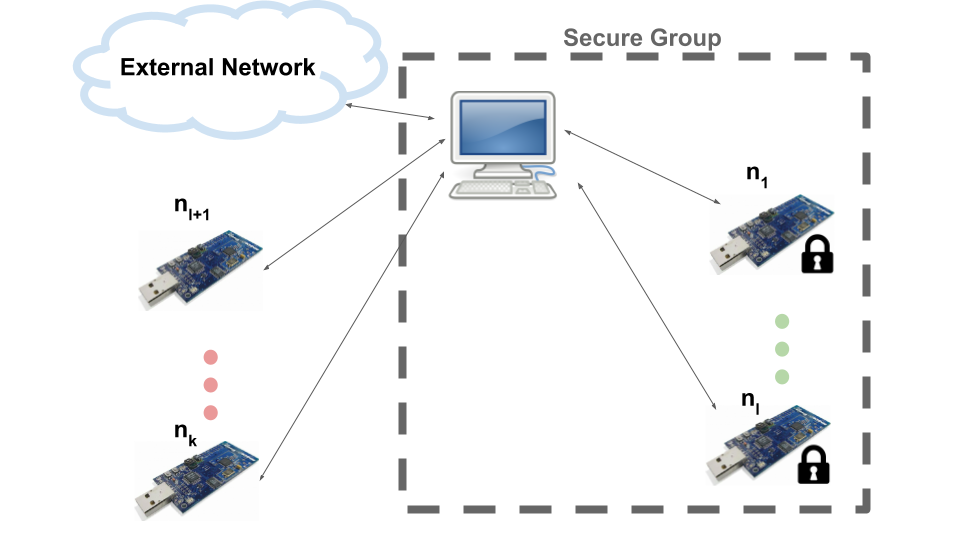
\includegraphics[width=5in]{images/network2.png}
\caption{Network Model. The network consists of a gateway and a set of nodes, supported by a communication infrastructure. All or a part of the nodes may be members of a group as shown in the figure (m nodes are in the group).}
\label{fig_network}
\end{figure}
Formally, the network can be modeled as a graph $Gr = \langle GW, N, E\rangle$ where \textit{GW} is the gateway that acts as a group initiator and manager and \textit{N} is a set of nodes $n_1, n_2, \dots, n_k$, and \textit{E} is the set of edges from \textit{GW} to $n_i$ representing bi-directional communication links.

\textit{GW} is considered a trustworthy entity which acts as  the group-manager which includes creating new groups, adding new nodes to the groups and maintaining the keys and the members of nodes of each group.
The gateway can be implemented according to a distributed architecture, providing benefits in terms of availability and robustness, avoiding to have a single point of failure on the single instance \textit{GW}.

It is also assumed that this communication technology and sensor nodes support  the transaction of multicast messages and is considered that all the entities in the network possess the same security associations and perform identical cryptographic functions. In our specific tests the entities support the following security functionality:
\begin{itemize}
\item Symmetric encryption scheme, specifically \acs{AES};
\item \acs{HMAC} function;
\item Hash functions, specifically SHA2.
\end{itemize}

\section{Code Implementation}
The proposed protocol consists of 2 important components: the nodes and the gateway.

The gateway and the nodes uses cryptographic operations: the decryption / encryption with AES, elliptic curve point multiplication and HMAC. As mentioned before, Tmote Sky has no support in hardware level for those cryptographic operations used by the proposed protocol. Thus, those cryptographic operations are implemented in application level using some existing C code examples with some modifications. As the consequence, the nodes and gateway memory occupancy and computing time may be higher compared to the case if the sensor supports those cryptographic functions in hardware level.

The module performing the basic elliptic curve point operations such as multiplication and addition is a C implementation based on $kmackay$'s $micro-ecc$.
This module include the ECDH and ECDSA functions and is an implementation for 8-bit microcontrollers.%%% CITATION https://github.com/iSECPartners/nano-ecc

For the implementation of the AES encryption algorithms with keys 192-bit long has been used a C implementation. %%%%%%%CITATION https://github.com/kokke/tiny-AES-c
The original module occupies relatively small memory and suitable for devices with little endian format.

The HMAC module is Software implementation in C of the FIPS 198 Keyed-Hash Message Authentication Code for SHA2 .
%%%%CITATION https://github.com/ogay/hmac

For the communication between the devices has been used the Rime communication stack. %CITATION RIME
Rime is a lightweight layered communication  stack for sensor networks created to simplify implementation of sensor network  protocols and facilitate code reuse.
Rime is already implemented in Instant Contiki 3.0 and has code footprint less than two kilobytes, with data memory requirements on the order of tens of bytes.


At the node's startup, a pair of private and public keys is generated and it start listening to broadcast connection to port 129. After receiving the Broadcast message from the gateway, each node start to listen on the port $146$ for unicast messages instead.


\begin{table}[H]
\caption{Node and Gateway Memory Usage [bytes] }
\label{nodeUsage}
\begin{center}
\begin{tabular}{|c|c|c|c|c|c|}
\hline
\textbf{Device} & \textbf{Text} &\textbf{Data} & \textbf{bss} & \textbf{dec} & \textbf{hex}  \\
\hline
Node & 26821 & 302 & 5524 & 32647 & 7f87\\
\hline
Gateway & 28077 & 302 & 5634 & 34013 & 84dd\\
\hline
\end{tabular}
\end{center}
\end{table}

In Table \ref{nodeUsage} we show the memory usage of the node and the gateway in bytes. 
\textit{text} shows the size of the code section in bytes (this will typically be in ROM).
\textit{data} and \textit{bss} show sections that contain variables, stored in RAM. 


